\documentclass{article}
% chktex-file 40
\usepackage[utf8]{inputenc}
\usepackage{amsmath}
\usepackage{amssymb}
\usepackage{tikz}
\usepackage{booktabs}
\title{Raul coss Bu}

\begin{document}

\textbf{Figura 4.1.} Forma gráfica del método de la transformada inversa.

embargo, si esta función inversa ya ha sido establecida, generando números aleatorios uniformes se podrán obtener valores de la variable aleatoria que sigan la distribución de probabilidad deseada.

\subsection*{Ejemplo 4.1. Distribución exponencial}

Se desea generar números al azar que sigan la siguiente distribución de probabilidad:

\begin{equation}
f(x) = \begin{cases}
\lambda e^{-\lambda x} & \text{si } x \geq 0 \\
0 & \text{si } x < 0
\end{cases} \tag{4.2}
\end{equation}

La distribución acumulada de esta distribución es:
\begin{equation*}
F(x) = \int_{0}^{x} \lambda e^{-\lambda t} dt = 1 - e^{-\lambda x}
\end{equation*}

y utilizando la ecuación (4.1), es decir, igualando la distribución acumulada con el número uniforme $R$, se obtiene:
\begin{align*}
1 - e^{-\lambda x} &= R \\
e^{-\lambda x} &= 1 - R
\end{align*}

Pero si $R$ sigue una distribución uniforme, entonces $1 - R$ también sigue esta distribución. Por consiguiente:
\begin{align}
e^{-\lambda x} &= R \nonumber \\
x &= -\frac{1}{\lambda} \ln R \tag{4.3}
\end{align}

\subsection*{Ejemplo 4.2. Distribución uniforme}

Se desea generar números al azar que sigan la siguiente distribución de probabilidad:
\begin{equation}
f(x) = \begin{cases}
\frac{1}{b-a} & \text{si } a \leq x \leq b \\
0 & \text{si } a > x > b
\end{cases} \tag{4.4}
\end{equation}

La distribución acumulada de esta distribución es:
\begin{equation*}
F(x) = \int_{a}^{x} \frac{1}{b-a} dt = \frac{x-a}{b-a}
\end{equation*}

e igualando esta expresión con el número uniforme $R$ se obtiene:
\begin{equation*}
\frac{x-a}{b-a} = R
\end{equation*}
\begin{equation}
x = a + (b-a)R \tag{4.5}
\end{equation}

\subsection*{Ejemplo 4.3. Distribución empírica}

Se desea generar números al azar que sigan la siguiente distribución de probabilidad:
\begin{equation}
f(x) = \begin{cases}
x & \text{si } 0 \leq x \leq 1 \\
1/2 & \text{si } 1 < x \leq 2
\end{cases} \tag{4.6}
\end{equation}

La distribución acumulada de esta distribución es:
\begin{align*}
F(x) &= \int_{0}^{x} t dt = \frac{x^2}{2} \text{ si } 0 \leq x \leq 1 \\
F(x) &= \frac{1}{2} + \int_{1}^{x} \frac{1}{2} dt = \frac{x}{2} \text{ si } 1 < x \leq 2
\end{align*}

puesto que la acumulada de la función tiene un valor de $1/2$ cuando $x=1$, entonces el valor de la variable aleatoria $x$ se determina de acuerdo a la siguiente expresión:

\begin{equation}
x = \begin{cases}
\sqrt{2R} & \text{si } R \leq 1/2 \\
2R & \text{si } R > 1/2
\end{cases} \tag{4.7}
\end{equation}

\begin{center}
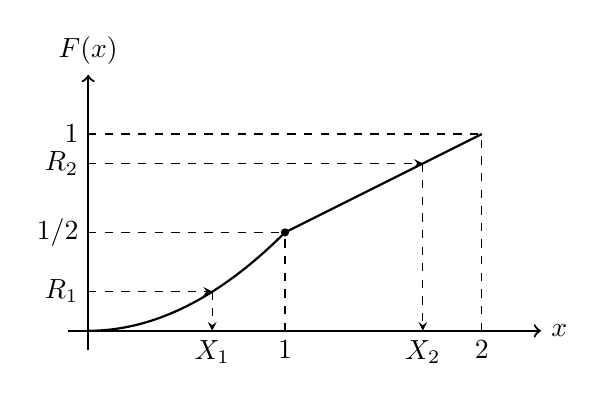
\begin{tikzpicture}[scale=2.5]
    % Ejes
    \draw[->, thick] (-0.1,0) -- (2.3,0) node[right] {$x$};
    \draw[->, thick] (0,-0.1) -- (0,1.3) node[above] {$F(x)$};

    % Curva f(x) = x^2/2 de x=0 a x=1
    \draw[thick, domain=0:1, smooth, variable=\x] plot ({\x}, {\x*\x/2});
    
    % Línea recta f(x) = x/2 de x=1 a x=2
    \draw[thick, domain=1:2, smooth, variable=\x] plot ({\x}, {\x/2});

    % Líneas de referencia principales (1 y 1/2)
    \draw[dashed] (0,1) node[left] {$1$} -- (2,1);
    \draw[dashed] (2,0) node[below] {$2$} -- (2,1);
    \draw[dashed] (0,0.5) node[left] {$1/2$} -- (1,0.5);
    \draw[dashed] (1,0) node[below] {$1$} -- (1,0.5);

    % Representación de R1 -> X1
    \draw[dashed, ->, >=stealth] (0,0.2) node[left] {$R_1$} -- (0.63,0.2);
    \draw[dashed, ->, >=stealth] (0.63,0.2) -- (0.63,0) node[below] {$X_1$};

    % Representación de R2 -> X2
    \draw[dashed, ->, >=stealth] (0,0.85) node[left] {$R_2$} -- (1.7,0.85);
    \draw[dashed, ->, >=stealth] (1.7,0.85) -- (1.7,0) node[below] {$X_2$};
    
    % Punto en el quiebre (1, 1/2)
    \filldraw (1,0.5) circle (0.5pt);
\end{tikzpicture}
\\ \textbf{Figura 4.2.} Distribución acumulada de la función (4.6).
\end{center}

\textbf{Tabla 4.1.} Distribución de probabilidad y distribución acumulada de la función $e^{-5} 5^x / x!${}.

\begin{center}
\begin{tabular}{ccc}
\toprule
$x$ & Distribución de probabilidad & Distribución acumulada \\
\midrule
0 & 0.0067 & 0.0067 \\
1 & 0.0337 & 0.0404 \\
2 & 0.0842 & 0.1246 \\
3 & 0.1404 & 0.2650 \\
4 & 0.1755 & 0.4405 \\
5 & 0.1755 & 0.6160 \\
6 & 0.1462 & 0.7622 \\
7 & 0.1044 & 0.8666 \\
8 & 0.0653 & 0.9319 \\
9 & 0.0363 & 0.9682 \\
10 & 0.0181 & 0.9863 \\
11 & 0.0082 & 0.9945 \\
12 & 0.0034 & 0.9979 \\
13 & 0.0013 & 0.9992 \\
14 & 0.0005 & 0.9997 \\
15 & 0.0002 & 0.9999 \\
\bottomrule
\end{tabular}
\end{center}

\textbf{Tabla 4.2.} Transformada inversa de la función $e^{-5} 5^x / x!${}.

\begin{center}
\begin{tabular}{c}
\toprule
    Si $0.0000 \leq R < 0.0067$, entonces $x=0$ \\
    Si $0.0067 \leq R < 0.0404$, entonces $x=1$ \\
    Si $0.0404 \leq R < 0.1246$, entonces $x=2$ \\
    Si $0.1246 \leq R < 0.2650$, entonces $x=3$ \\
    Si $0.2650 \leq R < 0.4405$, entonces $x=4$ \\
    Si $0.4405 \leq R < 0.6160$, entonces $x=5$ \\
    Si $0.6160 \leq R < 0.7622$, entonces $x=6$ \\
    Si $0.7622 \leq R < 0.8666$, entonces $x=7$ \\
    Si $0.8666 \leq R < 0.9319$, entonces $x=8$ \\
    Si $0.9319 \leq R < 0.9682$, entonces $x=9$  \\
    Si $0.9682 \leq R < 0.9863$, entonces $x=10$    \\
    Si $0.9863 \leq R < 0.9945$, entonces $x=11$    \\
    Si $0.9945 \leq R < 0.9979$, entonces $x=12$    \\
    Si $0.9979 \leq R < 0.9992$, entonces $x=13$    \\
    Si $0.9992 \leq R < 0.9997$, entonces $x=14$    \\
    Si $0.9997 \leq R < 0.9999$, entonces $x=15$    \\
\bottomrule
\end{tabular}
\end{center}

\subsection*{Ejemplo 4.4. Distribución Poisson}

Se desea generar números al azar que sigan la siguiente distribución de probabilidad:
\begin{equation}
f(x) = \frac{e^{-5} 5^x}{x!}, \quad x = 0, 1, 2, \dots \tag{4.8}
\end{equation}

Puesto que esta distribución de probabilidad es discreta, es necesario evaluar $f(x)$ para cada valor de $x$, y entonces determinar la distribución acumulada $F(x)$. Tanto la distribución de probabilidad como la distribución acumulada de esta variable aparecen en la tabla 4.1. De acuerdo a esta distribución acumulada, la tabla 4.2 muestra el valor que tomará la variable aleatoria $x$ dependiendo del intervalo al cual pertenece el número uniforme $R$.

\end{document}
    